\section*{The Eclipse ICE Item Project Generator}

\subsection*{Overview} 

This tutorial will teach you how you
can create your own ICE Items via the built in tools within ICE.  To demonstrate
these tools, we will walk through the development of an ICE Item project for the
FERN code, a fast efficient nuclear reaction network solver. 

So we don't have to worry about building Fern for this tutorial, we have
provided a convenient Docker image for Fern that you may use.  
This image must be apart of your local docker daemon images list for use in this
tutorial. You can add the image to your local Docker daemon in 2 ways: build the
image with the provided Dockerfile, or load the image through the image tar ball we have provided. To
build it from scratch, in the same directory as the Dockerfile, run 
\begin{lstlisting}[language=bash,caption={bash version}]
docker build -t eclipseice/fern .
\end{lstlisting}
To load the image from the provided tar ball, run 
\begin{lstlisting}[language=bash,caption={bash version}]
docker load < fernImage.tar.gz
\end{lstlisting}

After creating a new ICE Item plugin project, we will demonstrate how to
provide a few lines of code to get a Model Item showing in ICE that creates
input files for FERN. After that we will add a little code to the FERN
JobLauncher to be able to execute FERN locally, remotely, or via the
provided Docker image. 

Before we begin, make sure you have ICE cloned (Developer $>$ ICE $>$ Clone ICE)
into your workspace, and the provided Docker image loaded to your local Docker daemon. 

\subsection*{Creating a New ICE Item Plugin Project}
\begin{center} 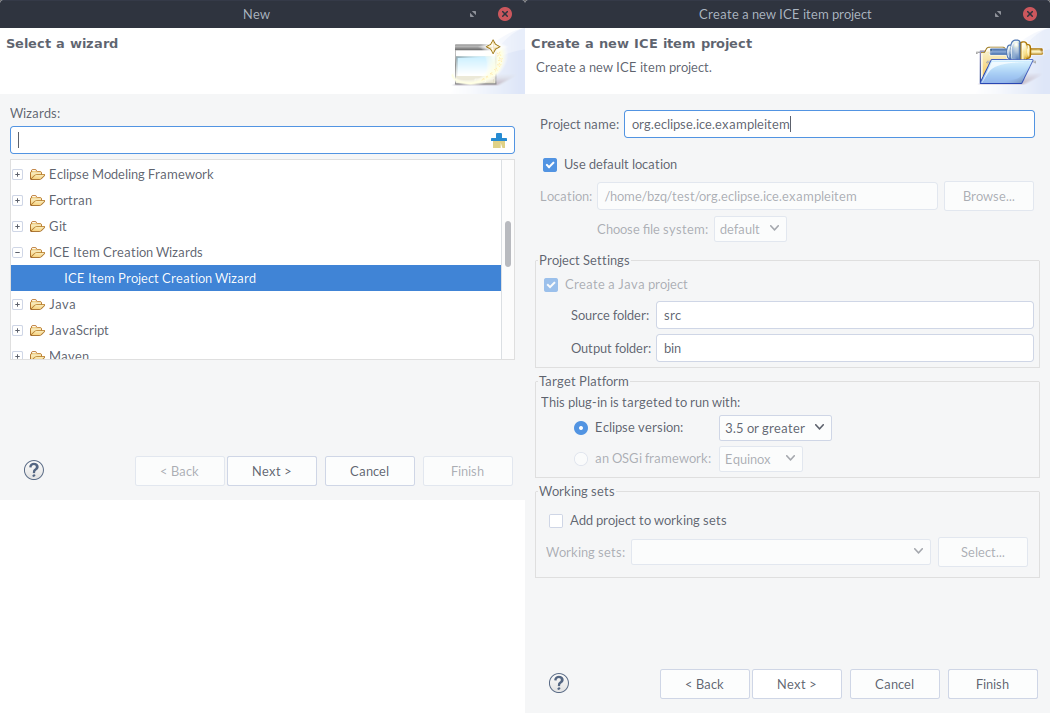
\includegraphics[width=\textwidth]{figures/comb12} \end{center}

To create a new ICE Item project, navigate to \texttt{File $>$ New $>$ Other}
and open the \texttt{ICE Item Creation Wizards} folder and 
select \texttt{ICE Item Creation Wizard}. You will be met with a standard new
project wizard page, in which you can name your project.  We will call ours
\texttt{org.eclipse.ice.fern}. Once you have named your project click the \texttt{Next >} button.
\begin{center} 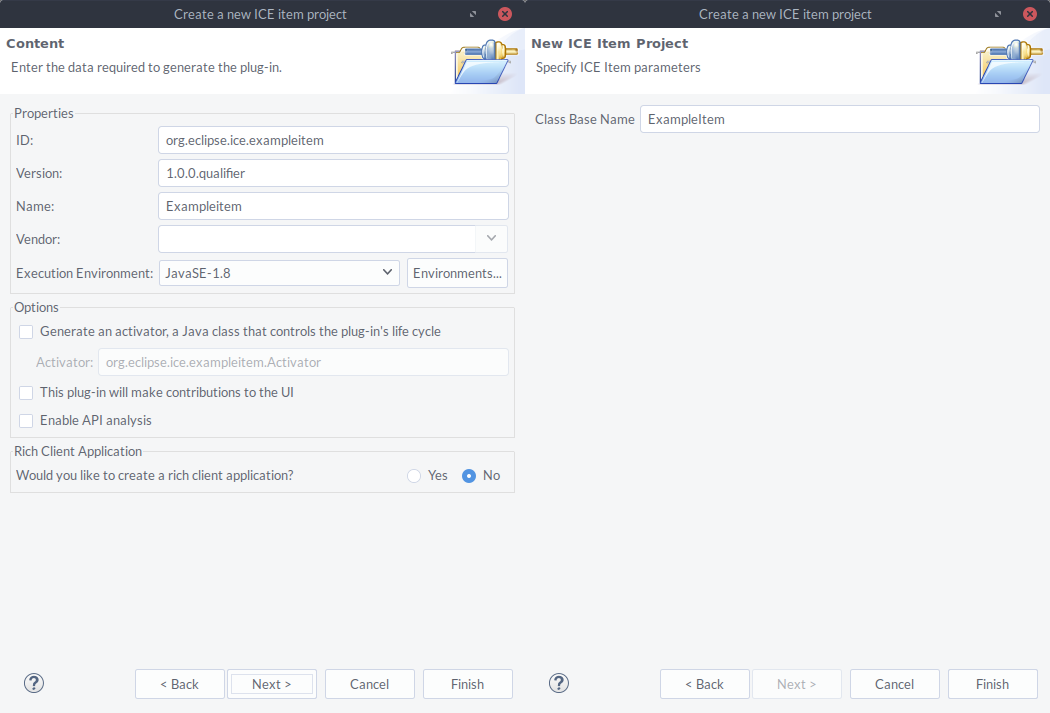
\includegraphics[width=\textwidth]{figures/comb23} \end{center}
Now you are able to customize the plugin-specific portions of the project. We do
not need an Activator to be generated, so uncheck that box, then select
\texttt{Next}. 

On this page you simply need to tell the wizard what you want to use as a base
name for your item classes.  We will call this one \texttt{Fern}. 
When you have entered your base class name you can
click the \texttt{Finish} button to generate your new ICE Item plugin project.

When the project has finished generating you should be able to explore the code
that has been created.  Within the source directory there will be two packages,
each containing two Java classes:

\begin{itemize} 
    \item \texttt{org.eclipse.ice.fern.launcher} 
    \begin{itemize}
        \item \texttt{FernLauncher.java} 
        \item \texttt{FernLauncherBuilder.java}
    \end{itemize} 
    \item \texttt{org.eclipse.ice.fern.model} 
    \begin{itemize} 
        \item \texttt{FernModel.java} 
        \item \texttt{FernModelBuilder.java}
    \end{itemize} 
\end{itemize}

To add functionality to the project you will only be responsible for editing
the \texttt{Launcher} and \texttt{Model} classes and can ignore the
\texttt{LauncherBuilder} and \texttt{ModelBuilder} classes.


\subsection*{Adding Functionality to the New Items}

\subsubsection*{The Fern Model}

The \texttt{FernModel} will be responsible for creating and
validating input parameters for FERN, in the form of a new FERN input file.  In
order to make the generated code run there are several pieces of information that need to be changed.  First, we
will need to set up the basic Item idenfification information. This information
is set in the setupItemInfo() method. Modify the writerName, readerName, and
outputName to match the following

\begin{lstlisting}[language=Java]
writerName = "INIWriter";
readerName = "INIReader";
outputName = "fern_config.ini";
\end{lstlisting}

We also need to provide a name, description, and export action name. The
generator will provide some default strings for these, but you may modify it
as you see fit. 

The name will serve as the display name for this Item, so set it
as \texttt{Fern Model}.
As for the description, this will also be used on the UI for the Item, so
provide some text like the following: \texttt{This Item constructs input files
for the FERN reaction network solver}. The export string will serve as the name
of the action that the user can select to write the provided data to file. Set
it to something like: \texttt{Export to INI}. You should now have a method that
looks like this:

\begin{lstlisting}[language=Java]
@Override
protected void setupItemInfo() {
	setName("Fern Model");
	setDescription("This Item constructs " +
	    "input files for the FERN reaction " +
	    "network solver"); 
	writerName = "INIWriter";
	readerName = "INIReader";     	
	outputName = "fern_output.ini";   
	exportString = "Export to INI";
	allowedActions.add(0, exportString);
}
\end{lstlisting}

The final line ensures that the export string is provided to ICE as an allowed
action, and displayed in the Item Process drop down.

With the identification information configured properly we can begin to
implement the Form for this Fern Model. This is done in the setupForm() method.
The generator has begun the process of implementing this method by instantiating
a Form for you to use, getting a reference to the IOService (which provides
IReader/IWriter realizations), and providing a commented out example of how to
fill out an ICE Form.

For this FERN input model, we want to add the following sections with data
entries: a network section with 
numSpecies, numReactions, numReactionGroups, massTol, fluxFrac, networkFile,
rateFile data entries, and initialConditions with T9, startTime, endTime,
initialTimeStep, and density. To achieve this for this Item, we will need to add
two \texttt{DataComponents}, one for the network section and another for the
initialConditions section. To each of those DataComponents we will add
appropriate IEntry instances for each of the data entries we have. 

Add the following to your setupForm() method: 

\begin{lstlisting}[language=Java]

    // Create the network section
    DataComponent networkComp = new DataComponent();
    networkComp.setName("network");
    networkComp.setDescription("The parameters needed " +
        "to describe the nuclear " +
    	"reaction network"); 
    networkComp.setId(1);
    
    // Create the IEntries we need for this DataComponent
    StringEntry numSpecies = new StringEntry();
    numSpecies.setName("numSpecies");
    numSpecies.setDescription("The number of species to consider");
    numSpecies.setDefaultValue("16");
    
    StringEntry numReactions = new StringEntry();
    numReactions.setName("numReactions");
    numReactions.setDescription("The number of reactions to consider");
    numReactions.setDefaultValue("48");
    
    StringEntry numReactionGrps = new StringEntry();
    numReactionGrps.setName("numReactionsGroups");
    numReactionGrps.setDescription("The number of reaction " + 
    	"groups to consider"); 
    numReactionGrps.setDefaultValue("19");

    StringEntry massTol = new StringEntry();
    massTol.setName("massTol");
    massTol.setDescription("The mass tolerance to consider");
    massTol.setDefaultValue("1e-7");
    
    StringEntry fluxFrac = new StringEntry();
    fluxFrac.setName("fluxFrac");
    fluxFrac.setDescription("The flux fraction to consider");
    fluxFrac.setDefaultValue(".01");
    
    FileEntry networkFile = new FileEntry(".inp");
    networkFile.setProject(project);
    networkFile.setName("networkFile");
    networkFile.setDescription("The network file for this problem");
    
    FileEntry rateFile = new FileEntry(".data");
    rateFile.setProject(project);
    rateFile.setName("rateFile");
    rateFile.setDescription("The rate file for this problem");
    
    networkComp.addEntry(numSpecies);
    networkComp.addEntry(numReactions);
    networkComp.addEntry(numReactionGrps); 
    networkComp.addEntry(massTol);
    networkComp.addEntry(fluxFrac);
    networkComp.addEntry(networkFile);
    networkComp.addEntry(rateFile);
    
    // Create the initial conditions section
    DataComponent initConditionsComp = new DataComponent();
    initConditionsComp.setName("Initial Conditions");
    initConditionsComp.setId(2);
    initConditionsComp.setDescription("The parameters " +
    	"needed to describe the	initial " + 
    	"conditions for the problem");
    
    StringEntry t9 = new StringEntry();
    t9.setName("T9");
    t9.setDescription("The temperature in Kelvin x 10^9");
    t9.setDefaultValue("7.0");

    StringEntry startTime = new StringEntry();
    startTime.setName("startTime");
    startTime.setDescription("The start time for the simulation.");
    startTime.setDefaultValue("1e-20");

    StringEntry endTime = new StringEntry();
    endTime.setName("endTime");
    endTime.setDescription("The end time for the simulation");
    endTime.setDefaultValue("1e-3");

    StringEntry initialTimeStep = new StringEntry();
    initialTimeStep.setName("initialTimeStep");
    initialTimeStep.setDescription("The initial time step " + 
    	"for the simulation."); 
    initialTimeStep.setDefaultValue("1.2345e-22");

    StringEntry density = new StringEntry();
    density.setName("density");
    density.setDescription("The initial density.");
    density.setDefaultValue("1e8");
    
    initConditionsComp.addEntry(t9);
    initConditionsComp.addEntry(startTime);
    initConditionsComp.addEntry(endTime);
    initConditionsComp.addEntry(initialTimeStep);
    initConditionsComp.addEntry(density);
    
    // Add the components to the Form
    form.addComponent(networkComp);    
    form.addComponent(initConditionsComp);
    
    // Set the Form ID info
    form.setName(getName());
    form.setDescription(getDescription());
    form.setId(getId());
    form.setItemID(getId());
\end{lstlisting}

Now we have a Form constructed for a typical FERN execution.

\subsubsection*{Fern Launcher}
The Fern Launcher handles the actual execution of the FERN application. The
generator creates the FernLauncher as a subclass of ICE's JobLauncher, which
provides a large array of features and functionality. As a subclass of
JobLauncher, the FernLauncher enables users to execute Fern locally, remotely,
or even through a Docker image. To do so, we just need to add a small amount of
code that customizes the ICE job launching capabilities for Fern. 

The first bit of code to add to the FernLauncher specifies the name of the
actual Fern executable. In the setupItemInfo() method, set the execCommand to
the following: 
\begin{lstlisting}[language=Java]
execCommand = "${installDir}fern-exec";
\end{lstlisting}
This tells ICE that the Fern executable is called \texttt{fern-exec}, and to
set the overall execution command to it's install path plus the executable name.

As for the Hosts information in the setupForm() method, let's simply change the
install path to what we know it will be in the Docker container we will use -
\texttt{/usr/bin}.
You can actually just change this on the Fern Launcher UI, but for efficiency, let's
do it here. 
\begin{lstlisting}[language=Java]
addHost("localhost", "linux x86_64", "/usr/bin");
\end{lstlisting}
We also need to inform the JobLauncher what other files are involved in this
execution. To do that, the JobLauncher provides an addInputType() method. Add
the following to setupForm():
\begin{lstlisting}[language=Java]
addInputType("Network File", "networkFile", 
			"Network File Description", ".inp");
addInputType("Rate File", "rateFile", "
			Rate File Description", ".data");
\end{lstlisting}

And that should be it.
The generator has taken care of everything else for us.
We are now ready to launch ICE with our Fern plugin, and use the Fern Items we
have just created.

\subsection*{Using the New Fern Items}
Now, using these new Items is easy. Simply open the Run Configurations wizard,
and open Eclipse Applications to see ICE launch configurations for Mac, Linux,
and Windows. Select the launch configuration for your OS and open the Plug-ins
tab. Scroll down to the \texttt{org.eclipse.ice.fern} plugin and turn it on for
this launch configuration. Then click Apply and Run. 

With a new ICE instance open, go to \texttt{File $>$ New $>$ Other} and select
the Create New Item Wizard. 
\begin{center} 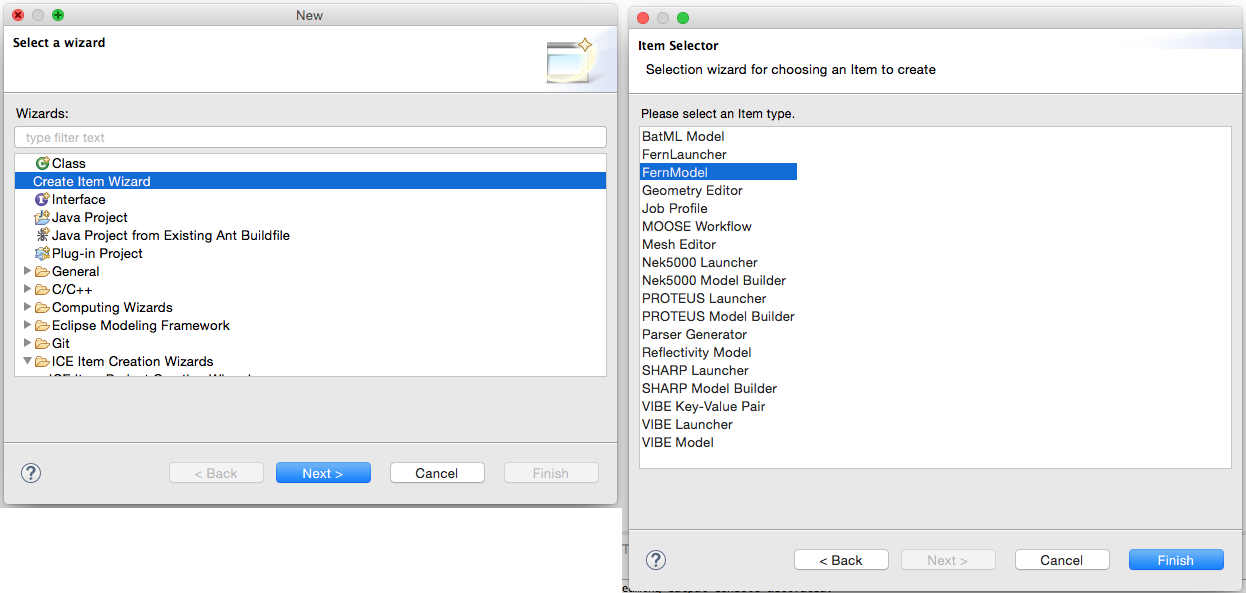
\includegraphics[width=\textwidth]{figures/creatingFernModelItem}
\end{center}
After selecting the FernModel Item, you will be presented with the view in the
figure below. 
\begin{center} 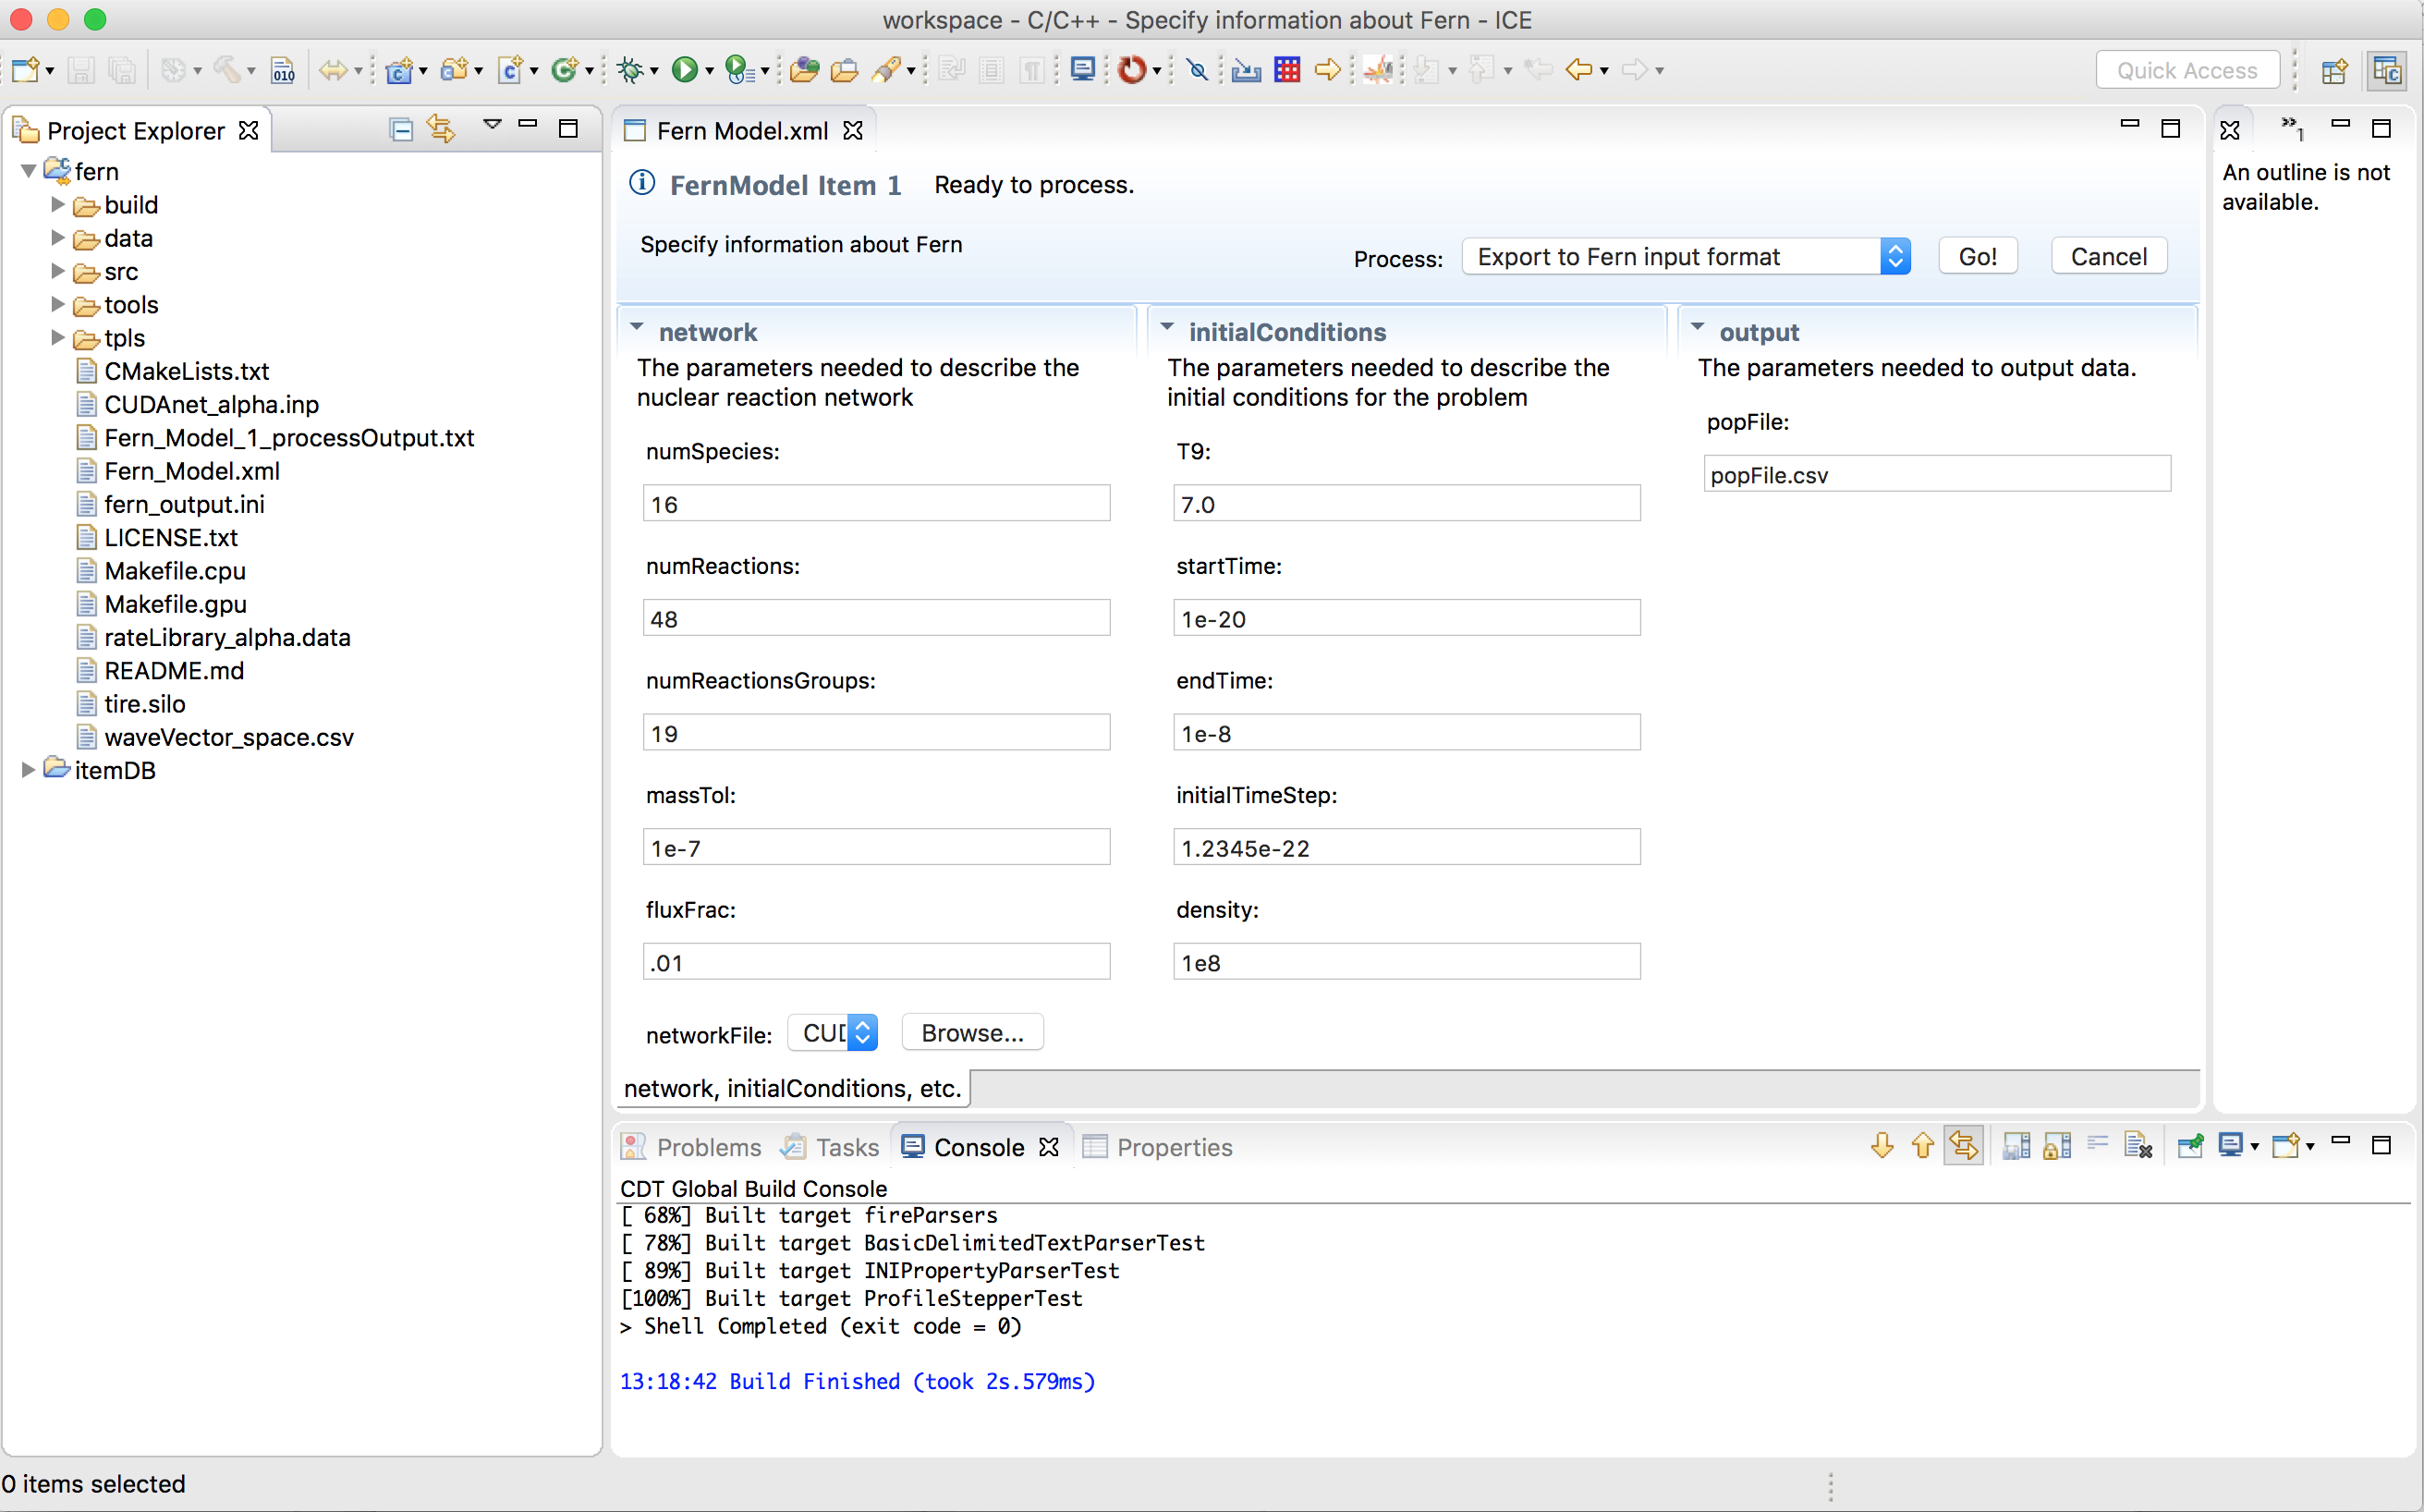
\includegraphics[width=\textwidth]{figures/fernmodelItem}
\end{center}
Here you can modify the various defaults with the values you would like for a
given Fern simulation. Once done, simply save the Item and click Go on the
Export to INI Process. This will execute the process of creating a new INI Fern
input file for use with the Fern Launcher. You can check the result by opening
the fern\_output.ini file, as shown below. 
\begin{center} 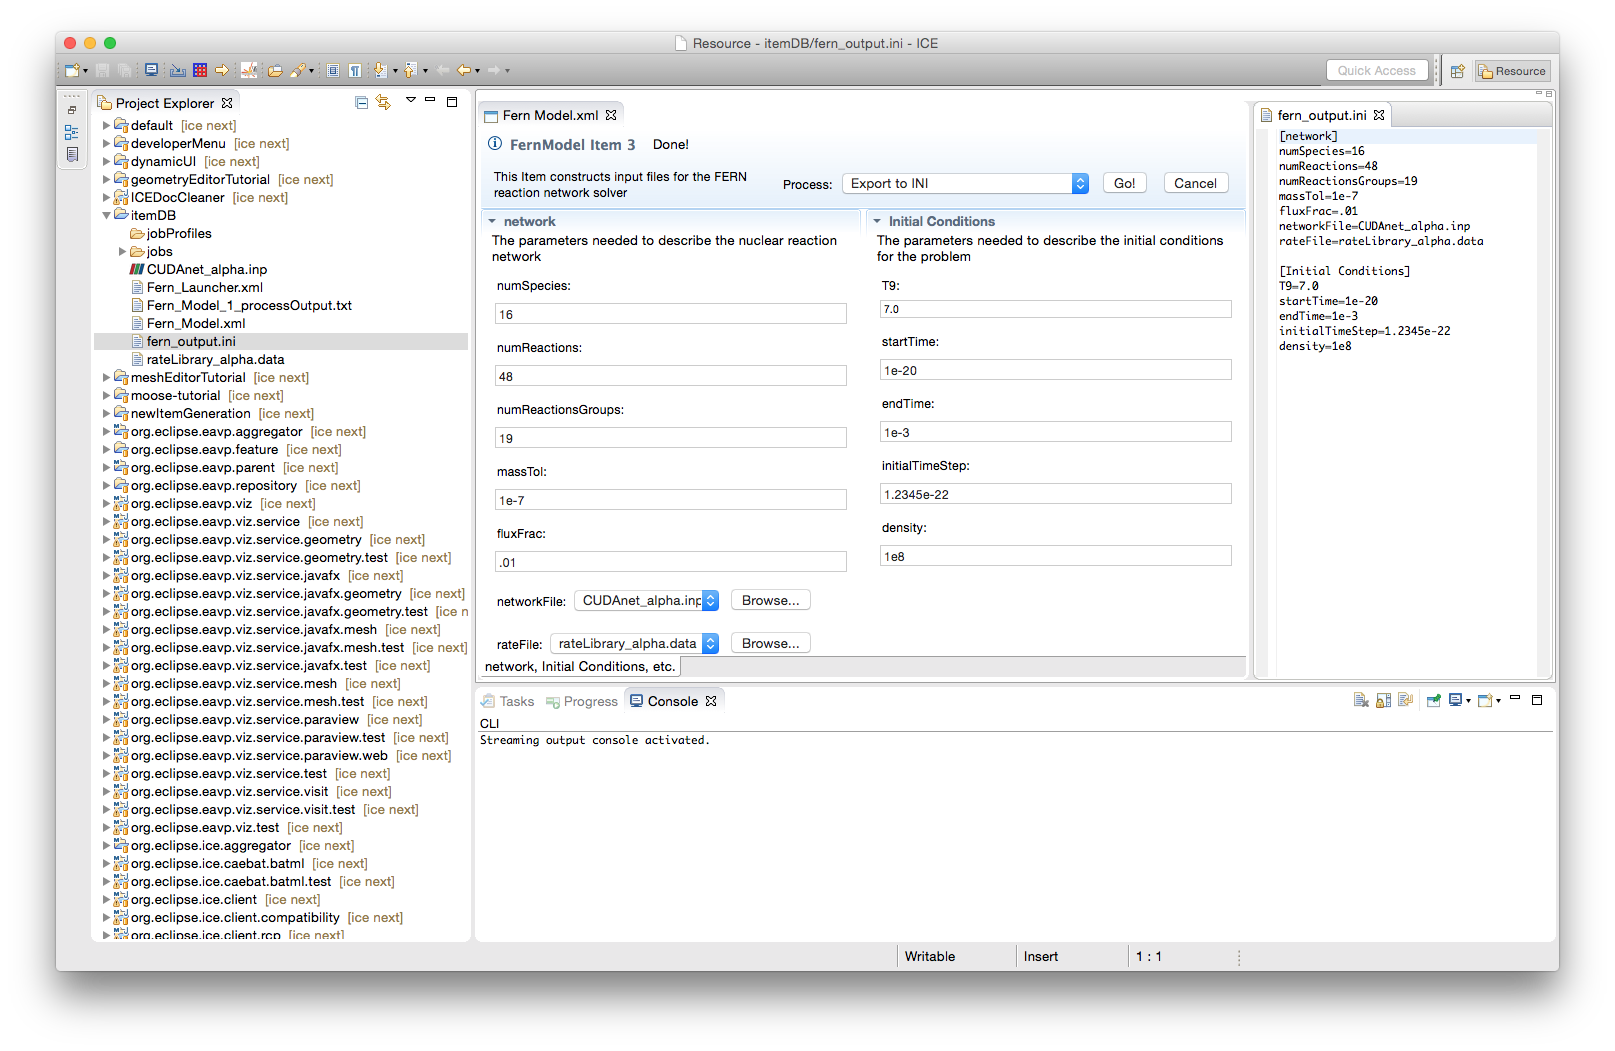
\includegraphics[width=\textwidth]{figures/result}
\end{center}

Now you can similarly create a new Fern Launcher. After creating the Launcher,
you should see a view like below. 
\begin{center} 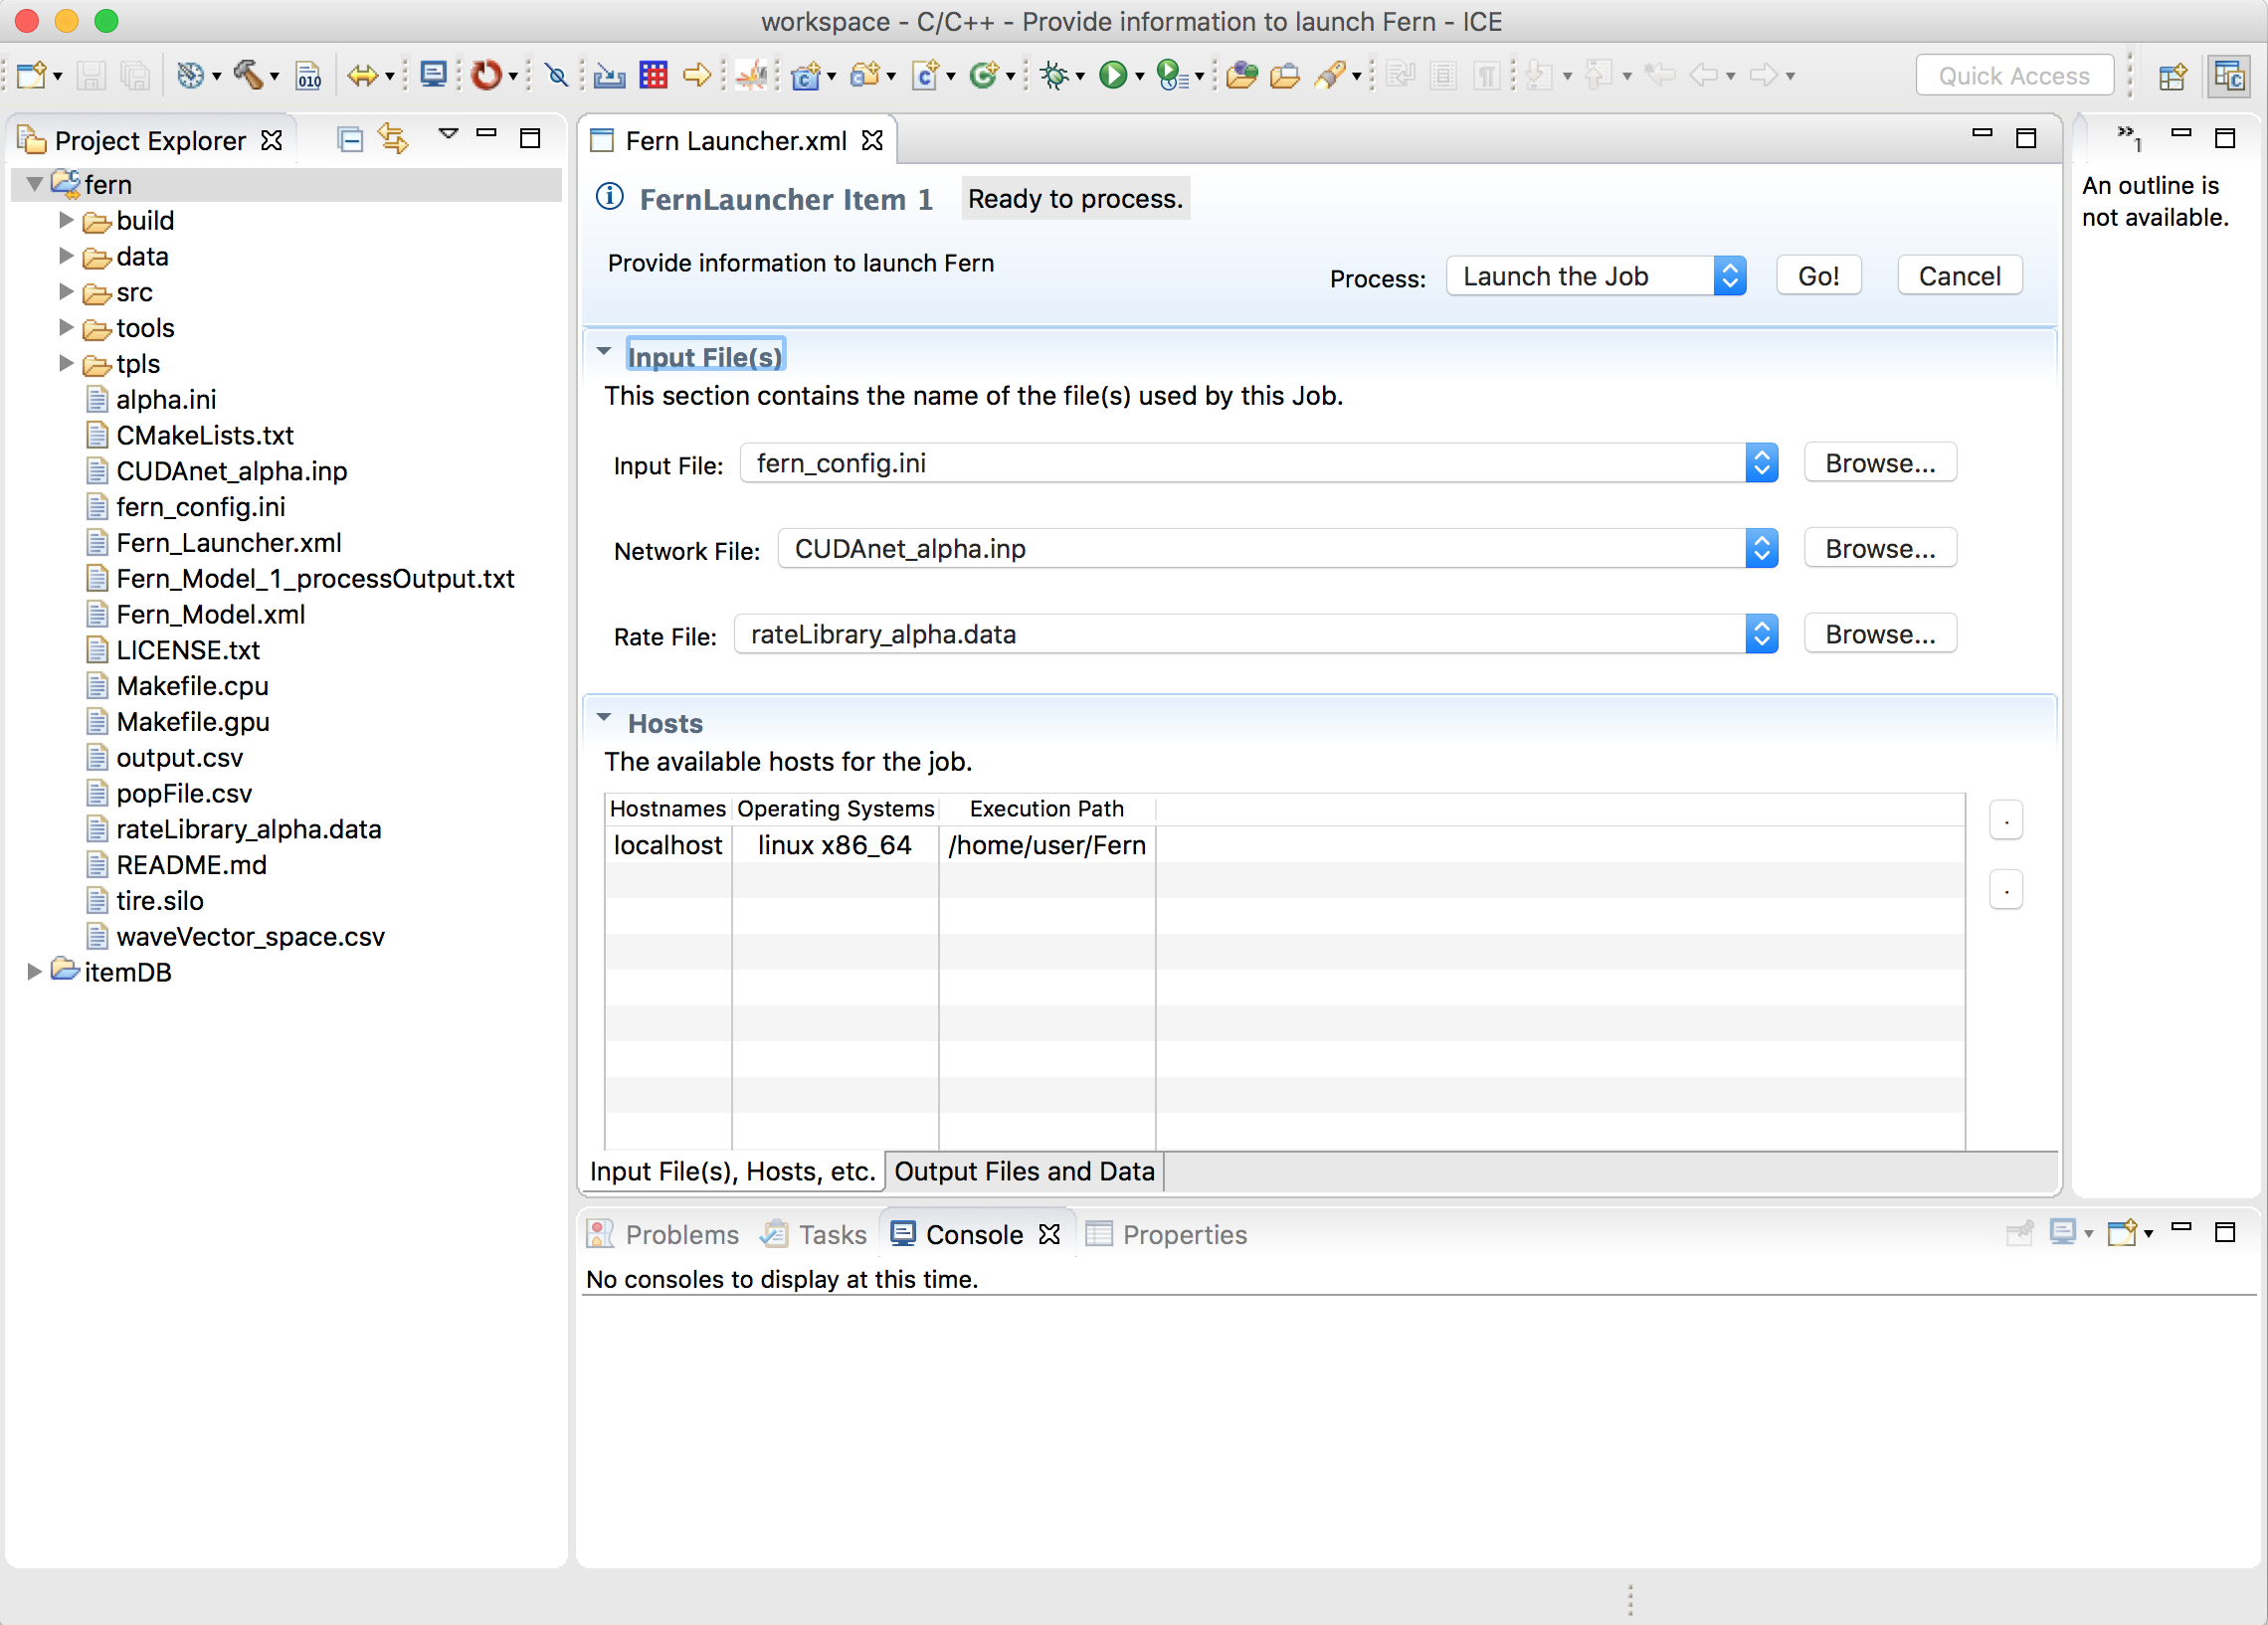
\includegraphics[width=\textwidth]{figures/launcher}
\end{center}
To configure a launch, simply set the correct
input file, along with its dependent network and rate files. 

At this point, if you had Fern built on your local machine, or if you had it
built on some remote host, you could configure that in the Hosts table. ICE
would then execute Fern based on that input. Since, for the purposes of this
tutorial, we don't have either of those configurations, we can use a third mode
of execution - launching our application via Docker. To do so, check the Launch
with Docker button, which will show a drop down widget populated with the list
of locally available Docker images. Select the eclipseice/fern image, and make
sure that the host table is configured to localhost and that the install path is
\texttt{/usr/bin}. Then simply launch Fern by clicking Go. This will pop up some
dialogs related to the connection of ICE to the Docker container, simply provide
a master password for Eclipse secure storage, and select yes on the known hosts
dialog. 

After the execution you should see the results in the Console, as shown below.
\begin{center} 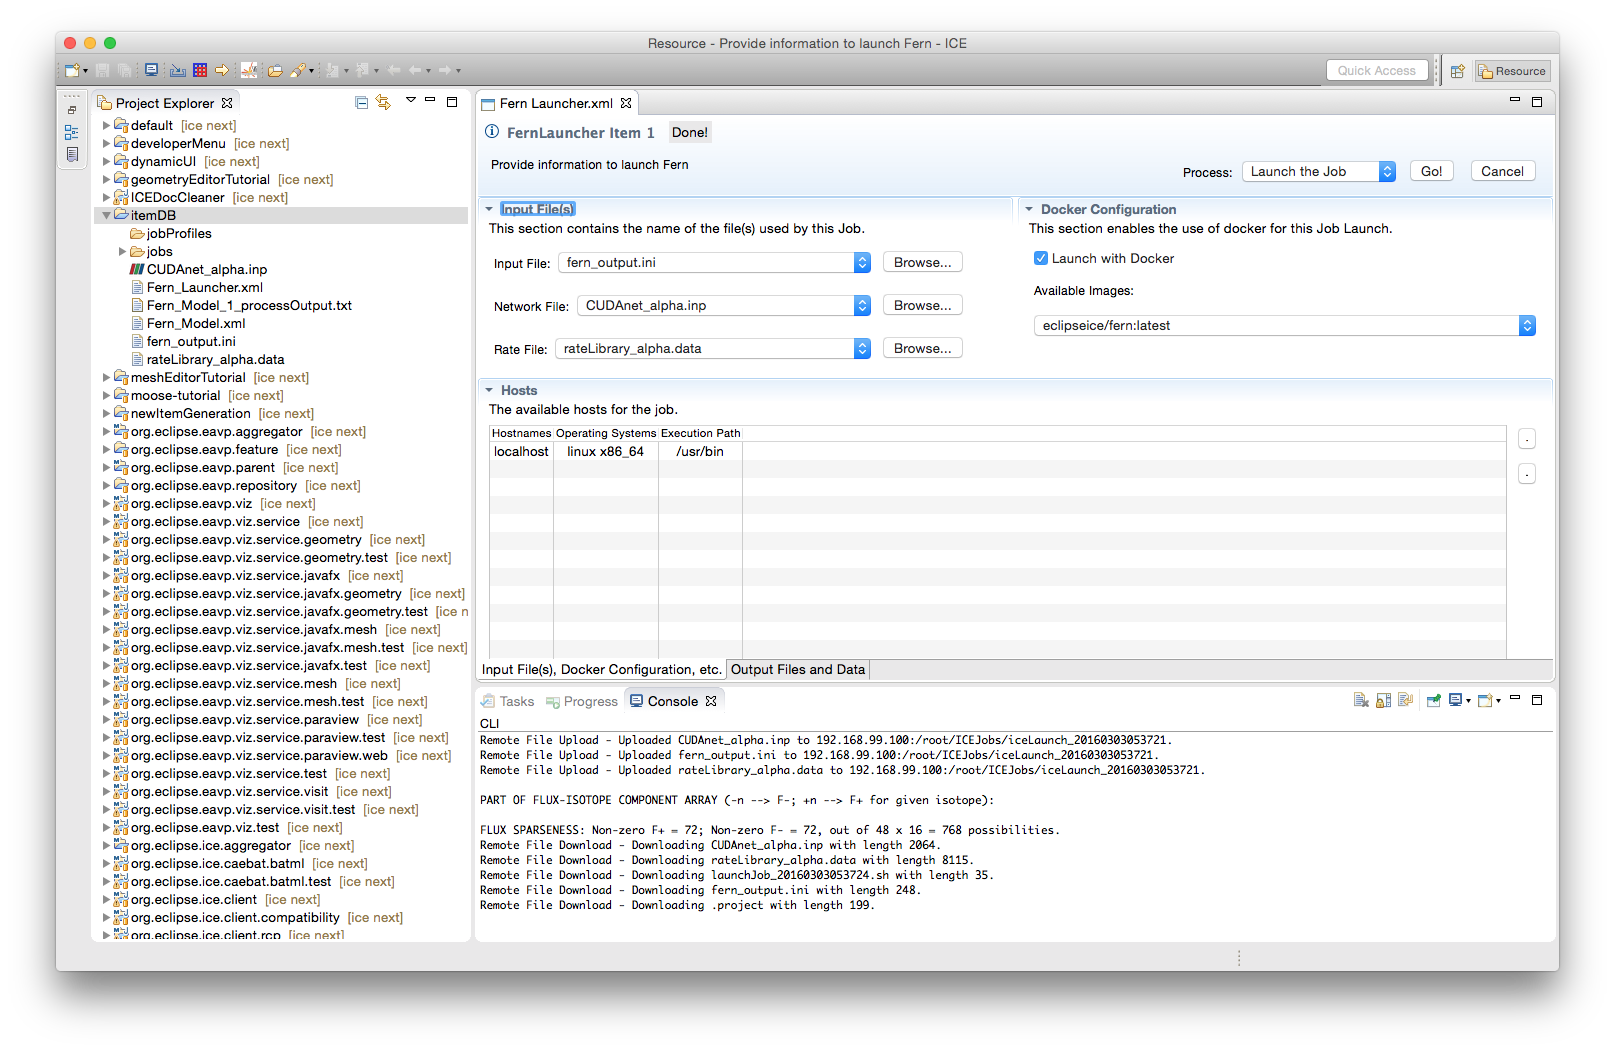
\includegraphics[width=\textwidth]{figures/launcherResult}
\end{center}